\documentclass[12pt,letterpaper]{article}

\usepackage{amsmath, amsthm, amssymb, amsfonts}
\usepackage{graphicx}
\usepackage{bm}

\theoremstyle{definition}
\newtheorem{dfn}{Definition}

\begin{document}

% The numbers below controls the amount of space between the following sections
\def\shiftdowna{0.32in}  % Adjust for balance
\def\shiftdownb{0.22in}  % Adjust for balance

\graphicspath{{./pictures/}}

% Set up the boiler plate at the top of the page

\begin{center}
\textbf{{\large Project Work Statement}}\\


% SPONSOR
\vspace \shiftdowna
\underline {Sponsor}\\ 
\vspace{5pt}
\textbf{{\large The RAND Corporation}}\\


% TITLE
\vspace \shiftdowna
\textbf{{\large Graphical models to explore the effects of globalization and development on prevalence of obesity}}



% SPONSORS
\vspace \shiftdownb
\underline {Participants}\\
\vspace{5pt}
Michael Weinberger, \texttt{michael.lee.weinberger@gmail.com} \\
\vspace{3pt}
\text{Zhendan Zhu}, \texttt{zhendanzhu@hotmail.com} \\
\vspace{3pt}
\text{Shannon Cebron}, \texttt{scebron@cis.jhu.edu}

% DATE
\vspace \shiftdowna
Date: \today

\end{center}

\vfill  
%Fill page to force following note to bottom


\newpage

\section{Background} 
Obesity is a medical condition identified by a Body Mass Index (BMI) (an adjusted proportion between height and weight) greater than 30. Obesity is proven to have extreme effects on a person`s quality of life \cite{health}. It is a major predictor in several potentially deadly types of disease; a common cause of physical degradation in the body manifested through pain in the joints and difficulty walking and moving; an aggravator of existing conditions such as sleep apnea and acid reflux disease; and a known detriment to mental health for reasons of body image and self-confidence.

When present in large proportions in populations, obesity is a major public health problem and a leading cause of preventable death. Treatment for heart disease, asthma, and diabetes is costly, driving up the cost of health care for the whole population. Furthermore, lost work hours due to obesity-related health problems detract from the health of the local economy.

As of 2010, the United States Center for Disease Control reports that 35.7 percent of the American population is obese, and this number has been steadily increasing since the 1960s \cite{prevalence}. The federal government estimates that up to USD 117 billion is lost yearly due to direct and indirect costs of such an obese population \cite{prevalence}.

The prevalence of obesity is increasing in countries around the world, at the highest rates in countries recently achieving highly developed status as according to the Human Development Index (a weighted average exceeding 0.8 between measures of education, life expectancy, and personal wealth). However, in some countries this effect is more pronounced than in others, and at this level of detail, the spread of obesity is not well-understood. It is surmised that through increased trade and increased personal disposable income, more processed food has become available around the world. Furthermore, rapid changes in technology have allowed nations to become more culturally integrated with one another, and some experts suggest that citizens of developing countries are becoming more and more influenced by the dietary and exercise habits of their developed neighbors.

A better understanding of the interplay between development, globalization, and obesity may contribute positively to efforts to prevent the spread of this preventable, expensive, and deadly disease.

The RAND Corporation is a public policy thinktank which conducts research and analysis to support political decision-making and the public good. Many elected persons agree that legislation may help to curb the obesity epidemic, and it is important that this legislation is designed in an informed, rigorous manner. By working with the RAND Corporation to conduct this project, we can help to give lawmakers insight into what factors most prominently affect obesity trends.

\section{Problem Statement}
% Consider the graph shown in Figure \ref{fig:stategraph}, which demonstrates the process by which our graphical constructs will be created, albeit on an
% international rather than regional scale. It is easy to see that the graph can elucidate information that hard data cannot.

Consider the following graph.

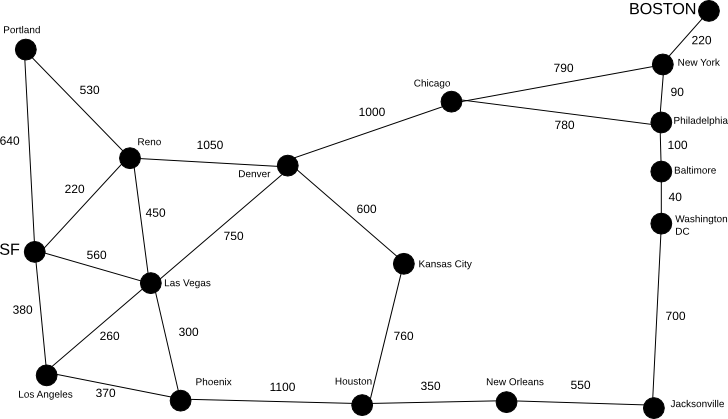
\includegraphics[scale=0.6]{graph_map_of_us.png}

This graph was constructed using major US cities as vertices and the distance in miles between the cities as edge lengths. Though the vertices in our model will represent nations, not cities, this is one example of how the graph might be structured.

The problem with inferring information from the graph is choosing how to define adjacencies, edge lengths, and vertex weights; in addition,
it must be decided which graphical properties will then be examined in a statistical model. Our task is to use sequential regression modeling to
investigate which properties are important predictors of national obesity rates, and use this information to inform our graph definitions and our final statistical models.

\section{Approach}
The proposed project consists of a few major components.

First, data needs to be acquired. A wealth of data is available from the CIA World Factbook, a reputable government-maintained website. Information can be
found on obesity rates, economic and trade data (such as GDP per capita, number of import/export partners, and income inequality), and national borders (numbers and names of bordering countries). This data will initially be handled in a data frame in either R or Python.

Secondly, the graphs need to be constructed. Both Python and Java offer fairly robust graphical structures and methods. Several different theoretical graphs will be created with a variety of definitions.

Thirdly, data will be extracted from the graphs. Measures such as neighborhood sizes, shortest paths, vertex degrees, and cliques and independent sets will be considered. This data will be tabulated and added to the original data frame.

Fourthly, a multiple linear regression model will be built to examine the appropriateness of a linear model for the data, as well as to give some initial insight into which variables are significant predictors of the national obesity rate. Predictor variables in this regression model will include items from the first step such as GDP per capita, and will also include items from the third step, e.g., number of developed countries within 1000 miles. The insights from this initial model will allow a more appropriate regression model to be designed, which may be non-linear or mixed in nature, depending on the results of the first model. This model will have a strong theoretical ability to predict the obesity rate in new countries not included in the original data, as well as give an effective account for the variation within the original data.

If time permits, then the graphical modeling stage will be revisited, with additional data considered, such as information about food market and international restaurant chain presence.

If data on past obesity rates is not readily available, then the project will be scaled down to exclude the model to predict future obesity rates, since for this model data is needed from more than one point in time. In this case, the current obesity rate model will be expanded to consider more data that otherwise would only have been included with time permitting.
  
\section{Milestones}
We have the following major deadlines:
\begin{itemize}
    \item Work Statement due date, Sep 28, 2012,
    \item Midterm Presentation due date, Oct 17, 2012,
    \item Progress Report due date, Oct 26, 2012,
    \item Final Presentation due date, Nov 6, 2012,
    \item Final Report due date, Nov 30, 2012.
\end{itemize}

\section{Deliverables}
\subsection{From Team to Sponsor} % (fold)
The following outputs are expected from this project:
\begin{itemize}
    \item Regression model that accurately predicts current obesity rate 
    \item Regression model that accurately predicts future obesity rate
    \item R package with complete documentation and usage examples
    \item Technical report and presentations summarizing the work. 
\end{itemize}

\subsection{From Sponsor to Team} % (fold)

In order for our project to be a successful one, we will need:
\begin{itemize}
    \item Requests for specific data to be included in the model
    \item Computing resources
    \item Nations of high interest to be examined in more detail
    \item Timely responses to inquiries
    \item Symposium attendance travel expenses
\end{itemize}


\newpage

 \begin{thebibliography}{1}

  \bibitem{health} Stanford Hospital and Clinics. {\em Health Effects of Obesity.}  2012: Stanford University.

  \bibitem{prevalence}  CDC Division of Nutrition, Physical Activity and Obesity. {\em Adult Obesity Facts} 2010:
  United States Center for Disease Control.

  \end{thebibliography}

\end{document}
